% Based on the ACM SIG Proceedings sample. The KDD Research CFP specifies
% sigconf,anonymous,review. Overleaf root document: main.tex.
% The original vector overview is PDF 1.7.
\ifdefined\pdfminorversion\pdfminorversion=7\relax\fi
\documentclass[sigconf,anonymous,review]{acmart}
\setcopyright{none}
\acmDOI{}
\acmISBN{}
\acmConference[KDD 2027 Research Track]{KDD 2027 Research Track}{August 2027}{San Jose, CA, USA}
\acmBooktitle{Manuscript prepared for the KDD 2027 Research Track}
\acmYear{2027}
\usepackage{amsmath}

\begin{document}
\title[Which Analyses Can Agent-Generated Cohorts Support?]{Which Scientific Analyses Can Agent-Gener\-ated Biomedical Cohorts Support?}
\author{Anonymous Author(s)}

\begin{abstract}
Published studies can report how often two biomarkers cross thresholds while leaving their continuous association uncertain. Can a scientific agent turn that evidence into individual records useful for a specified analysis? We ask agents to read original biomedical articles, choose joint probability laws and author executable samplers without target participant records. We apply the same analyses to the resulting cohorts and to measured samples. In two controlled tasks, adding joint evidence reduced discrepancy for the analysis it informed, while the four companion discrepancies increased. In a prospective iron-status experiment, three independent sessions recovered a crude anemia odds ratio of 6.65 from eight published strata. Seven executable agent laws passed 16 checks against the source. Their odds ratios ranged from 6.55 to 6.86, but their hemoglobin--ferritin rank correlations ranged from $-0.272$ to $0.446$. In an external survey, 44 women had complete measurements. Their weighted rank correlation was 0.069, with a wide interval, and no woman crossed the low-ferritin threshold required to estimate the odds ratio. A separate prospective blood-pressure experiment found that two laws with identical published moments implied different joint screening rates. These experiments trace each downstream conclusion to the published evidence, the model chosen by the agent, and the measurements available for verification.
\end{abstract}

\ccsdesc[500]{Computing methodologies~Modeling and simulation}
\ccsdesc[300]{Applied computing~Life and medical sciences}
\keywords{scientific agents, synthetic biomedical data, joint distributions, evidence synthesis, analysis utility}
\maketitle

\section{Introduction}
A study in rural northern China reports anemia counts across eight combinations of iron, folate and vitamin B$_{12}$ status~\cite{zhu}. A researcher with no access to those individual records wants a virtual cohort of US women. She intends to use the same records for two questions. How much higher are the odds of anemia among women with low ferritin? How closely do hemoglobin and ferritin track each other across their continuous ranges? An agent can answer the first question \emph{for the source study} by collapsing the eight rows into four cells. Any assignment of continuous measurements within those cells preserves that answer. Many such assignments give different answers to the second question. Moving from the Chinese study to the US population introduces a further uncertainty, even for the first question.

This example motivates an evaluation of scientific agents in which the deliverable is a dataset. A researcher specifies a population, measurements and intended analyses. The agent reads the evidence, chooses how to model the relationships that the publications leave open, and delivers a program that can draw complete records. The researcher can then run regressions, compare subgroups or apply screening rules. These are concrete uses when records are costly to collect or unavailable. Their value depends on the analysis one plans to perform.

Previous work has shown how to generate synthetic cohorts using shared fitted models, aggregate tabulations, trial curves and published covariates~\cite{filshtein,llmsynthor,synthipd,kmgen}. Our question concerns the point where scientific modeling discretion enters this process. Two agents can reproduce the same table by writing different sampling laws. A single law can reproduce a regression slope and miss the dependence that governs a screening rule. We therefore evaluate one \emph{analysis in one population} at a time. We keep the analysis code fixed when changing its input and trace the resulting estimate back to the article and the authored program.

We make three contributions. First, we document a whole-cohort generation workflow in which the agent performs the numerical interpretation and authors the sampling law. We audit six constructions from original papers, including source arithmetic and the assumptions carried into executable code. Second, we isolate the contribution of joint evidence in two biomedical tasks. Both targeted discrepancies fall, while the four companion discrepancies increase. A matched-size resampling experiment places a separate lifestyle reconstruction on the scale of variation between two samples of measured records. Third, we prospectively elicit alternative laws in two settings. In blood pressure we check which screening rates five source moments allow. In iron status we start from an original article and compare second models against the same sealed primary. In each case we record the laws and their predicted sensitivities before inspecting a new survey.

\section{From a research request to executable records}
\label{sec:method}

\begin{figure*}[t]
\centering
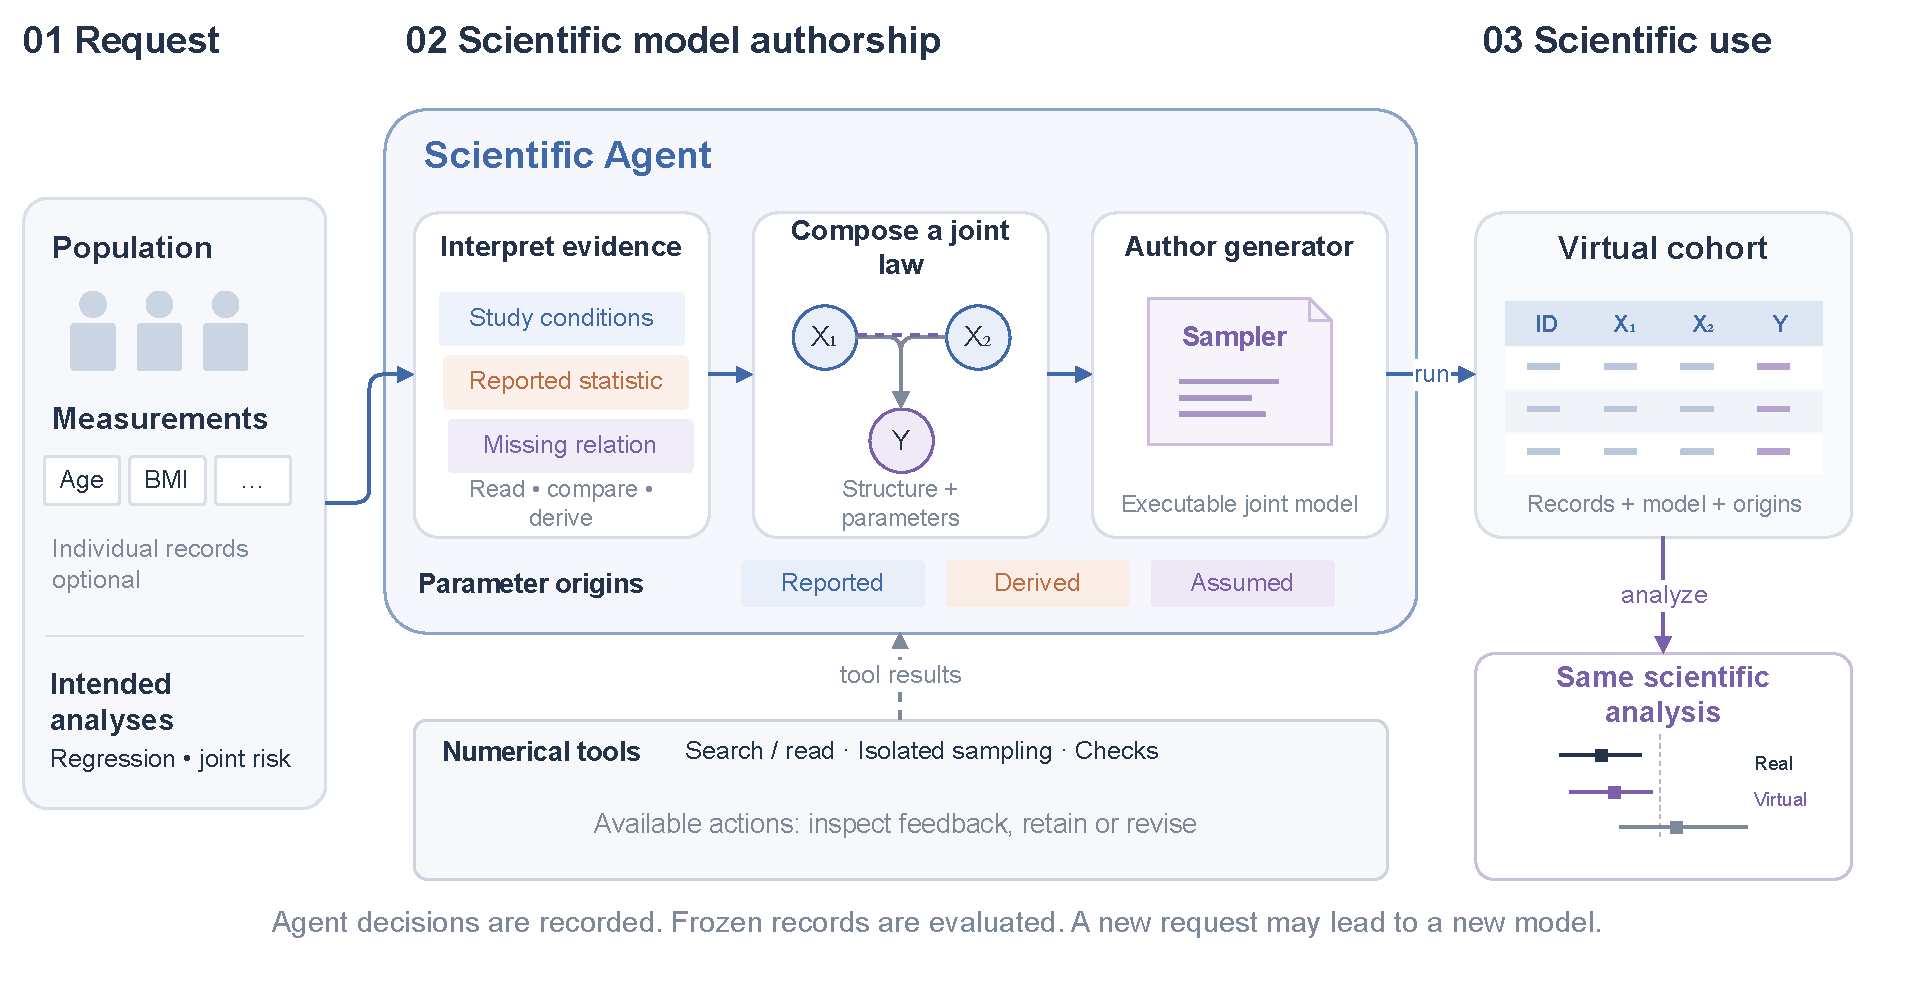
\includegraphics[width=.96\textwidth]{figures/method.pdf}
\caption{The researcher supplies a target population, measurements and analyses. The agent reads and interprets evidence, chooses a joint law and authors the sampler. The execution service draws the records. A separate evaluator runs the requested analyses. In the whole-cohort experiments, the individual-record input on the left is empty.}
\Description{Left to right, a research request specifies a population, variables and analyses. A scientific agent interprets studies and produces a sampling program. The program produces virtual records for scientific analyses.}
\label{fig:method}
\end{figure*}

\paragraph{Scientific contract.}
A request names the unit of observation, population, measurement units and intended analyses. For example, the iron request calls for continuous hemoglobin and ferritin in nonpregnant US women aged 20--44. We disclose the analyses to the constructor so it can seek appropriate evidence. The measured target records and their analysis results stay with the evaluator. Figure~\ref{fig:method} also covers enrichment of existing records. The experiments reported here generate complete records from zero target participant inputs.

Write $s_j(P_j)$ for a statistic evaluated under the population, measurement and adjustment rules of source study $j$. A paper reports a rounded estimate of this quantity. The researcher's question is an analysis $a(P_T)$ in target population $T$. Even exact knowledge of $s_j(P_j)$ generally leaves open both the shape of the source distribution and the correspondence between $P_j$ and $P_T$. We use this distinction in two ways. We compare a generated estimate of $a$ with the same estimate in a measured sample. Where source summaries permit several laws, we can also ask whether varying the law changes $a$ while preserving those summaries.

\paragraph{Agent and execution service.}
In the initial original-paper experiments (Section~\ref{sec:original}), each fresh model session received a starting paper, the request, tools for reading and supplementary retrieval, an output schema and an execution budget. The agent could inspect source tables and methods, resolve units, propose a dependence structure, and choose numerical parameters. It returned an executable sampler, its parameters and a record of consequential choices. It could inspect a trial draw and submit a revision. The execution service validated the interface, ran the submitted program in isolation and recorded its identity and seeds. The coordinator supplied the task and starting article. The constructor selected the scientific law. The final rows were sampled from that law. The study therefore tests authorship of a reusable generator from an assigned paper. Each of the two articles was assigned to three sessions.

\paragraph{Audit of a modeling decision.}
For each quantity we record what the source reported, how the agent transformed it and how the code used it. We separately record any change of population or statistical definition. For example, a partial correlation can be exactly derived from a source matrix while its use as a residual correlation after additional adjustment remains an assumption. We check the submitted program against the account of the model choice and independently recompute scientific estimates. This audit can establish that a model implements its stated choice. Only evidence on the requested analysis can establish how useful that choice was.

\paragraph{Evaluation.}
Each constructor commits its program before the final draws. Draws with different seeds measure variation conditional on that program. Separate constructors can express different modeling choices. For each task we run a single estimator implementation on generated records and the measured reference under the relevant sampling design. For the published lifestyle analysis, this is a reimplementation of the reported regression. A reference value estimates a quantity in a measured sample and carries uncertainty. Where a user-defined tolerance is absent, we report differences in their native units and describe the scientific use they support.

\section{Can the agent model what the paper reports?}
\label{sec:original}
We ran three fresh sessions on each of two requests using the same recorded GPT configuration. All six located the relevant table in the assigned original article, performed a numerical derivation, authored a whole-cohort generator, inspected one simulated trial and retained the first candidate. Each law produced three final draws. The 18 tables contain 72,000 simulated records. Independent computation reproduced all 99 draw-level analysis and diagnostic estimates to within $7.6\times10^{-14}$. Construction used 142 model calls at an estimated token tariff of US\$1.51. These counts describe six modeling decisions.

\begin{figure*}[t]
\centering
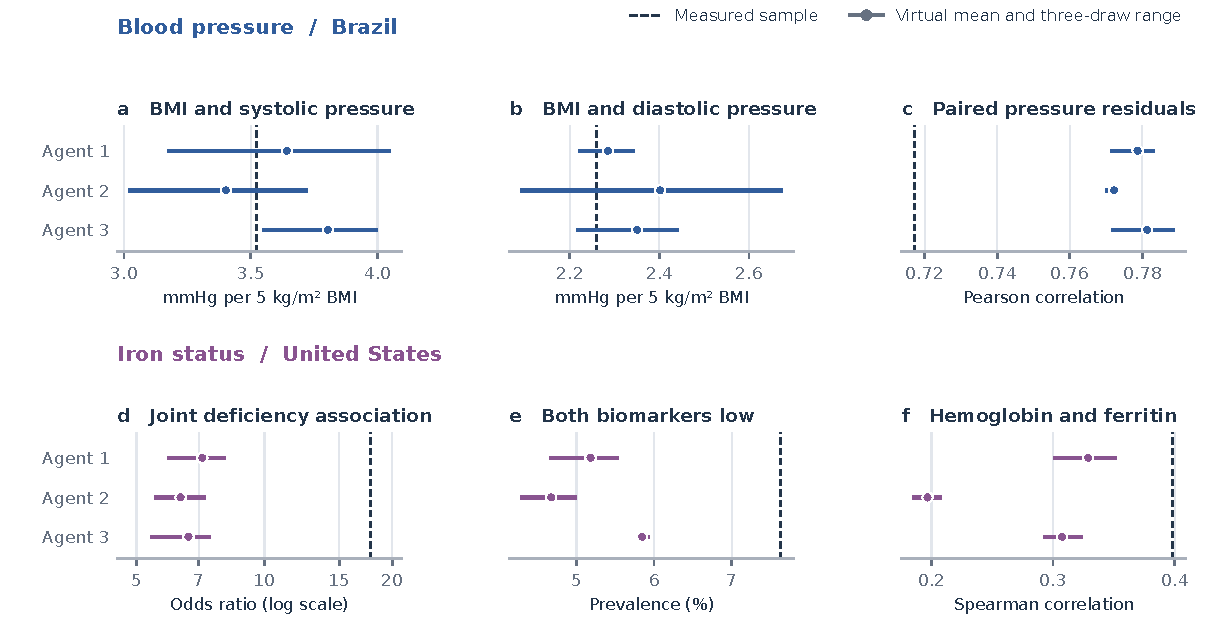
\includegraphics[width=.96\textwidth]{figures/original-paper.pdf}
\caption{The same analysis run on virtual and measured records. Each point is one constructor's mean across three seeded draws. The segment spans those draws. Dashed lines are measured sample estimates. Each panel has its own scale. The systolic slopes are near the Brazilian estimate. The iron odds ratios cluster around the value derived from the Chinese source paper, well below the US estimate.}
\Description{Six panels compare three constructors with a measured reference. The three systolic slopes straddle the reference, all diastolic slopes and residual correlations exceed it, and all three iron odds ratios, joint prevalences and rank correlations fall below their reference.}
\label{fig:original}
\end{figure*}

\paragraph{Blood pressure.}
The assigned article studied partnered adults aged at least 40 in rural Burkina Faso~\cite{jaspert}. Its correlation matrix gives the associations of age, body mass index (BMI), systolic blood pressure (SBP) and diastolic blood pressure (DBP). Each agent combined its entries to obtain the source age- and BMI-adjusted residual correlation, approximately 0.788. The source also reports BMI regression coefficients from a more extensively adjusted model. The agents used positive diastolic and pulse pressures and summed them to obtain systolic pressure. They chose different demographic distributions and conditional pressure levels. This construction enforces the physical ordering of the two pressures for every draw.

We applied the target regressions to virtual records and compared them with estimates from 8,352 eligible participants in the Brazilian National Health Survey (PNS)~\cite{pns}. The age- and sex-adjusted systolic slope ranged from 3.40 to 3.80 mmHg per five BMI units, bracketing the measured 3.52. The corresponding diastolic slopes were 2.29--2.40 versus 2.26. The pressure correlation after adjusting for age, sex and BMI was 0.772--0.781 versus 0.717. All three laws also yielded wider pressure distributions than the measured sample (Appendix~\ref{app:profiles}). Thus a user could recover the direction and approximate scale of these BMI associations while overestimating dependence between the paired measurements.

\paragraph{Iron status.}
Of the women in the source table, 173 had both markers low, 85 had only low hemoglobin, 331 had only low ferritin and 1,082 had neither~\cite{zhu}. Each agent computed the crude odds ratio, $(173\times1082)/(85\times331)=6.65$, and distinguished it from the paper's adjusted odds ratio of 6.448. One agent then used a Clayton copula to couple continuous biomarker values. Another modeled two latent iron-store components and a change in hemoglobin response below a threshold. The third used a saturating response with inflammatory and other-anemia components. Supplementary evidence informed marginal assumptions. All three authors noted an ambiguity in the source's ferritin labeling.

We evaluated crude threshold odds, joint prevalence and rank correlation against survey-weighted US National Health and Nutrition Examination Survey (NHANES) estimates from 979 eligible women~\cite{nhanes}. The thresholds were hemoglobin $<12$ g/dL and ferritin $<15$ $\mu$g/L. Generated odds ratios were 6.35--7.14, close to the source's 6.65. The measured US odds ratio was 17.79. All three programs preserved a positive association and substantially understated its strength in this comparison. For the same records, the prevalence of both low markers was 4.67--5.85\% versus 7.63\%, and Spearman correlation ranged from 0.197 to 0.329 versus 0.398 (Figure~\ref{fig:original}). A correct table extraction can therefore coexist with appreciable error after population transfer.

\paragraph{What does direct arithmetic already give the researcher?}
Five times the published BMI coefficients gives 3.75 mmHg for SBP and 2.20 mmHg for DBP in the source's fully adjusted model. Those two numbers provide informative comparisons with the Brazilian slopes, even before simulation. Likewise, the four iron counts yield the crude odds ratio and a joint-low prevalence of 10.35\% for the Chinese study. They supply no continuous rank correlation. For that question, choosing how to populate the four cells with continuous values is the scientific modeling step. Comparing the three authored programs makes that choice visible.

\section{What changes when the agent gets joint evidence?}
\label{sec:controlled}
We held the research request and modeling interface fixed within each task and changed the supplied evidence. Three fresh constructors worked in each of three conditions per case, with three final seeds per constructor. The first condition provided the common base. For pressure, this already contained previously published relationship evidence. For iron status, it supplied study context. The second condition added single-variable summaries from the selected source. The third added a joint block \emph{from the same source sample}. This consisted of six pairwise correlations for pressure, or the paired low-marker counts for iron. The latter two conditions differed only in that block. No target feedback or programmed numerical relationship entered these comparisons.

\begin{table}[t]
\caption{Mean absolute discrepancy by evidence condition. The last two columns differ only in the joint source block. Lower is closer to the measured sample within each row.}
\label{tab:evidence}
\centering
\begin{tabular}{@{}lrrr@{}}
\toprule
Requested analysis & Base & Marginal & Joint\\
\midrule
BP residual correlation & .1632 & .1633 & \textbf{.0350}\\
BMI--SBP slope & .1934 & .3396 & .5091\\
BMI--DBP slope & .7276 & .7378 & .7550\\
Iron log odds ratio & 1.5495 & 1.7620 & \textbf{.9373}\\
Both markers low (pp) & 1.7903 & .5187 & 2.5940\\
Iron rank correlation & .0769 & .0447 & .1736\\
\bottomrule
\end{tabular}
\end{table}

Table~\ref{tab:evidence} reports discrepancies for every requested analysis. We computed the absolute error for each draw and averaged first across seeds, then equally across constructors. The two pressure slopes are in mmHg per five BMI units. The iron odds ratio is evaluated on the natural-log scale. Adding the matrix reduced residual-correlation error from 0.1633 to 0.0350. Adding the four-cell table reduced log-odds-ratio error from 1.7620 to 0.9373. The two other pressure estimates and the two other iron estimates moved farther from their respective sample references. In particular, the joint table identifies a threshold association in its source sample but gives neither the target prevalence nor the within-cell ordering needed for continuous ranks. These results identify the change across the tested evidence conditions. Their magnitude is descriptive across three constructors per condition.

\section{A prospective test with two compatible laws}
\label{sec:prospective}
Before inspecting paired outcome values in a new Freetown screening release~\cite{freetown,freetowndata}, we specified two analyses: the unadjusted Pearson correlation of SBP and DBP, and the fraction simultaneously reaching 140 mmHg systolic \emph{and} 90 mmHg diastolic. The latter is a conjunction of two thresholds. It has a different interpretation from a clinical hypertension diagnosis. The agent received five rounded source summaries from the rural Burkina Faso study~\cite{jaspert}, comprising means 125.22 and 80.54 mmHg, standard deviations 18.22 and 10.98 mmHg, and raw correlation 0.78. It also received the target sampling context. This experiment starts from extracted summaries. The earlier experiments in Section~\ref{sec:original} test original-paper reading.

\begin{figure*}[t]
\centering
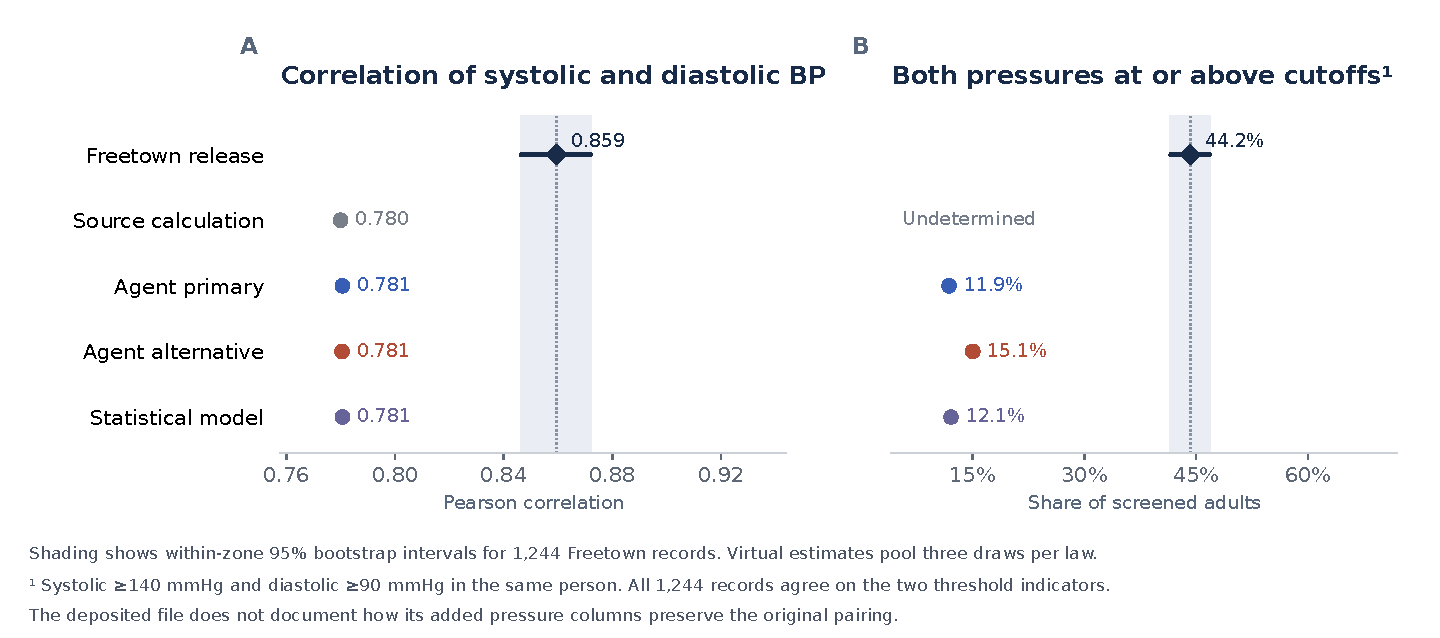
\includegraphics[width=.94\textwidth]{figures/freetown.pdf}
\caption{Prospective screening test. The source correlation is available by direct calculation. The joint threshold probability depends on the model. Points for the two agent laws and the statistical comparator are estimates from seeded virtual draws. The band describes uncertainty for the deposited Freetown sample conditional on the represented zones. The extreme target threshold result led to a separate audit of the deposited fields.}
\Description{Two panels show a released correlation of 0.859 and a joint threshold percentage of 44.2. Three virtual arms give correlations near 0.78 and threshold percentages between 11.9 and 15.1.}
\label{fig:freetown}
\end{figure*}

One fresh agent was asked to propose a primary and an alternative law and state which analyses the source constrained. Before disclosure, it identified the correlation as reported, the joint threshold as underdetermined and the application to a new population as uncertain. Its primary model coupled positive DBP and pulse pressure with a bivariate lognormal law. A statistical comparator specified in advance from the same five numbers independently used this family. The agent's alternative was a 75:25 mixture. It separated the component means and subtracted their between-component contribution from the within-component covariance. These are hypothetical population structures. Both laws preserve all five working moments, including an exact population correlation of 0.780.

Independent numerical integration of the fixed programs gave joint threshold probabilities of 11.9449\% and 15.0851\%. These two examples establish a 3.14 percentage-point difference consistent with the five summaries. They give a lower bound on the range of answers permitted by those constraints. The full range may be wider. A separately prespecified finite-draw criterion asked whether the simulated gap, after subtracting four times the sum of Monte Carlo standard errors, exceeded two percentage points. The adjusted gap was 1.60 points, below the criterion. We report both results because they answer different questions.

After the freeze we analyzed the deposited fields of 1,244 eligible screening participants aged 40 or older. Their correlation was 0.859 (within-zone bootstrap 95\% interval 0.847--0.872), and 44.21\% met both thresholds (41.64--46.79\%). All three simulated arms were far below the released joint rate (Figure~\ref{fig:freetown}). A post-disclosure count clarified how to interpret that difference. Of the eligible records, 550 met both thresholds, 694 met neither, and neither isolated exceedance occurred. The same pattern held across all 2,394 released records. The codebook identifies the component fields as added variables. Their pairing history remains unresolved. The measured discrepancy applies to the deposited fields. The unresolved pairing limits its biological interpretation.


\section{Which iron analyses survive a change of model?}
\label{sec:ironpros}
We repeated the prospective test from the full Chinese iron-status article~\cite{zhu}. This time the target was adult nonpregnant, nonlactating mothers in rural Burkina Faso~\cite{burkina_iron}. Three fresh GPT sessions each submitted a primary generator. For each primary, two further sessions received the same article, research request and sealed program. One was asked for a second defensible model. The other was asked for a model that would expose the sensitivity of a requested analysis. A fixed statistical comparator independently sampled within the published categories. All constructors could see the scientific questions. The Burkina Faso measurements stayed with the evaluator.

The paper also reports ferritin geometric means and depletion frequencies across three hemoglobin bands. All three primary authors extracted the four crude counts correctly. All seven completed authors predicted that the source odds ratio was determined and that the rank correlation was sensitive. After a documented parameter-interface correction, the seven laws passed all 16 prespecified source checks (Appendix~\ref{app:ironpros}). Across the same virtual records, the odds ratio stayed near 6.65, while choices about ordering people within hemoglobin bands changed the continuous correlation. Four of six planned primary--alternative pairs completed. In all four, the rank gap exceeded its estimated simulation noise. Only one primary yielded both alternatives, which limits the prompt comparison.

\begin{figure*}[t]
\centering
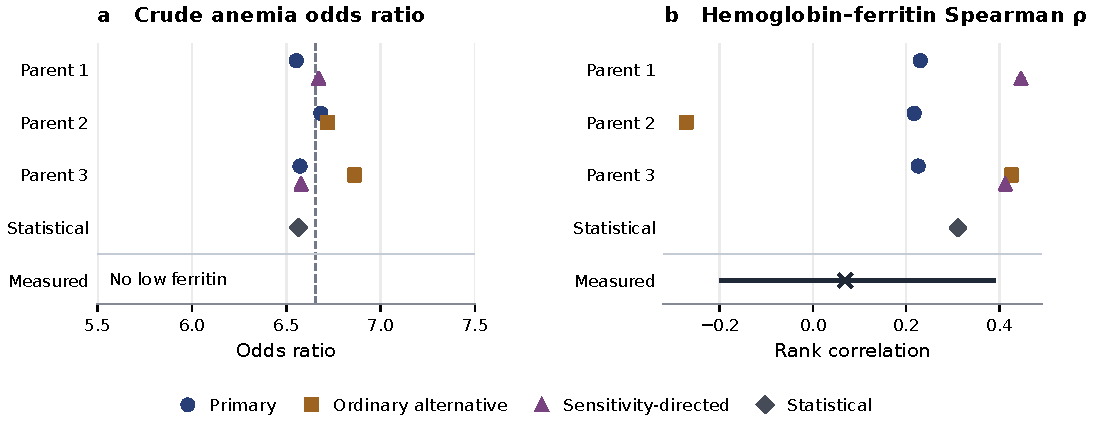
\includegraphics[width=.98\textwidth]{figures/iron-alternatives.pdf}
\caption{Two analyses on each sealed iron cohort. Symbols in each parent row distinguish the primary law and the two alternative requests. Two requests reached the output limit and have no point. The dashed line marks the source odds ratio of 6.65. The measured row gives the survey-weighted result for 44 women. The rank interval resamples villages within province. No woman in this sample had low measured ferritin.}
\Description{Agent odds ratios cluster between 6.55 and 6.86. Their rank correlations range from minus 0.272 to plus 0.446. The measured rank correlation is 0.069, with a wide interval.}
\label{fig:ironpros}
\end{figure*}

For one parent the ordinary alternative changed the rank correlation from $0.217$ to $-0.272$. Its author chose a within-band Gaussian copula parameter of $-0.75$, an explicit sensitivity assumption with no measured support in the source. Two positive-dependence alternatives for another parent moved its correlation from $0.226$ to $0.426$ and $0.413$. Even the positive scenarios gave different effect sizes. Appendix~\ref{app:ironproof} shows why this freedom survives the group summaries.

After all draws and source checks were sealed, 44 women had complete paired measurements across 23 villages. The measured survey-weighted rank correlation was 0.069 (95\% village-bootstrap interval $-0.198$ to $0.389$). No participant met the ferritin threshold, and 18 met the hemoglobin threshold. The external odds ratio was unestimable. Both thresholds agreed with the release's own flags in all 44 records. Figure~\ref{fig:ironpros} shows what the source supports and what the verification sample can resolve. The source odds ratio was reproducible, several continuous relationships remained possible, and the new sample distinguished them imprecisely.

\section{How large is the gap relative to sampling variation?}
\label{sec:lifestyle}
Two real samples from the same study need not give the same regression coefficient. We used that observation to interpret a source-rich reconstruction of the Turkana lifestyle study~\cite{lea,leadata}. Two independent agents generated age, sex, lifestyle, BMI, total cholesterol and high-density lipoprotein (HDL) cholesterol, with three draws of 1,226 rows each. We reimplemented the original age- and sex-adjusted comparison once and applied it to both measured and virtual records. The same study supplied the evidence and the measured reference, making this an analysis-reconstruction experiment.

In 500 repetitions, we drew two real resamples and one resample from each of the six saved virtual tables, matching trait-specific sample sizes and counts by sex and lifestyle. For urban versus pastoralist BMI, the mean absolute difference between real resamples was 0.316 kg/m$^2$. Across the six virtual tables, virtual--real differences were 0.314--0.428 kg/m$^2$. For the rural versus pastoralist comparison, the virtual effect was too small by 7.80--9.55 mg/dL for total cholesterol and by 4.07--6.21 mg/dL for HDL. The measured cholesterol standard deviations were 42.81 and 20.23 mg/dL. Virtual-resample means were 31.49--32.67 and 14.50--14.89. A researcher rehearsing the urban BMI contrast would thus get a recognizable result. A researcher planning a study whose precision depends on lipid variability would be relying on distributions that were too narrow. Figure~\ref{fig:lifestyle} shows all nine contrasts. Appendix~\ref{app:lifestyle} gives their numerical values.

\begin{figure*}[t]
\centering
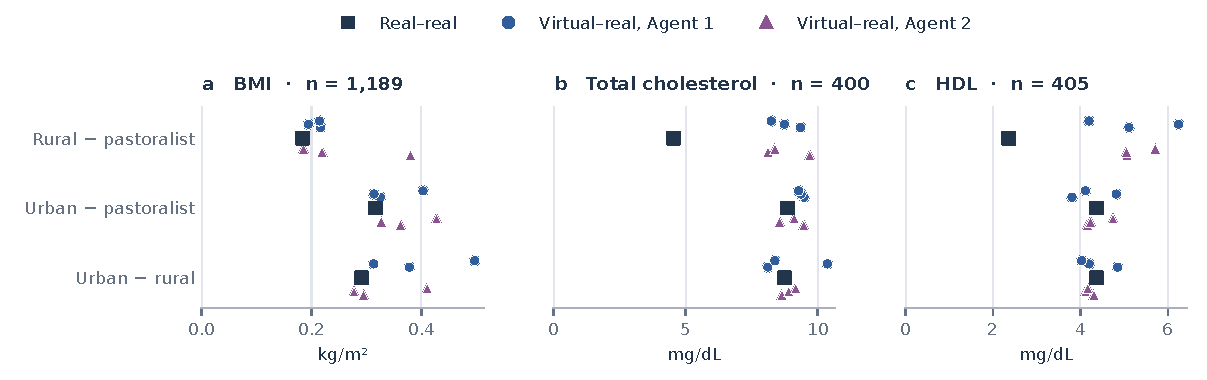
\includegraphics[width=.92\textwidth]{figures/lifestyle.pdf}
\caption{Matched-size mean absolute discrepancies for all nine adjusted lifestyle contrasts. The real--real estimate comes from two resamples of measured records. The virtual--real estimates use six saved virtual tables from two constructors. Native units and sample sizes differ across panels.}
\Description{Three panels compare BMI, total cholesterol and HDL across rural, urban and pastoralist lifestyles. Virtual versus real discrepancies are similar to real versus real for the urban BMI contrast, and larger for both rural lipid contrasts.}
\label{fig:lifestyle}
\end{figure*}

\section{Related work}
G-Sim uses an LLM to propose and revise simulators with numerical calibration~\cite{gsim}. LLMSynthor constructs micro-records aligned with macro statistics using discrepancy-guided generation~\cite{llmsynthor}. Filshtein et al.\ generate synthetic cohorts by sharing fitted models~\cite{filshtein}. SynthIPD reconstructs individual trial data from reports, and KMGen uses a skill-based agent for synthetic patient data from survival and adverse-event evidence~\cite{synthipd,kmgen}. SynthCraft supports healthcare data access and augmentation~\cite{synthcraft}. These works establish substantial prior art for both agentic simulation and generation from publications. Our experiments follow an agent's scientific choices into several estimands on the same output and compare each with an independently computed measured-sample analysis. The experiments supply a task-specific comparison of laws under identical information in Sections~\ref{sec:prospective} and~\ref{sec:ironpros}.

Statistical approaches can incorporate external summary information from heterogeneous populations~\cite{syndi}. The fact that moments leave other functionals partially identified has a long history~\cite{bounds}. Our prospective experiment uses an agent to construct and execute two examples and asks what this ambiguity means for a specific screening analysis. Work on inferential utility also shows that treating synthetic observations as measured records can understate uncertainty~\cite{inferential}. Here the virtual rows approximate the consequences of an assumed law. Model choice, source sampling variation and population transfer remain separate sources of uncertainty.

\section{Discussion}
An agent can do substantive scientific modeling from a published table. In these experiments it chose adjustments, reconstructed a threshold odds ratio, selected a continuous joint law and produced analyzable records without seeing target outcomes. What the records support depends on the statistic. The Brazilian systolic slopes preserved an interpretable effect scale. The iron models recovered the direction and strength of the \emph{source} threshold association while understating its strength in the US sample. Joint source evidence improved the scientific analysis it directly informed in both controls. It also shifted other quantities that the added evidence left open.

A practical use follows. Deliver a sampled cohort together with the generator and an analysis-by-analysis statement of the source calculation, assumptions and transfer evidence. For a published odds ratio alone, direct arithmetic is sufficient. The generated records become informative when a researcher applies a second analysis or examines how that analysis changes across compatible laws. In Freetown, the two laws exposed a three-point model choice before disclosure. The much larger external discrepancy then prompted scrutiny of the measurements themselves.

The scope is bounded. PNS and NHANES were previously analyzed during development. Fresh constructors were screened from target values, but one pressure session saw and excluded a same-survey search preview. Turkana resamples share one measured pool. The prospective pressure result relies on one constructor and a release with unresolved field provenance. The iron result relies on three parents, two incomplete alternatives, and a small measured sample with no iron-depleted women. Both prospective tests used one GPT configuration. Clinical use would require domain review of the alternative laws and external samples with adequate precision and event counts. For the studies reported here, the defensible product is a virtual cohort accompanied by an explicit account of which scientific analyses the evidence can sustain.

\bibliographystyle{ACM-Reference-Format}
\bibliography{references}
\appendix
\section{Construction, data and reproducibility}
\label{app:design}
\paragraph{Original papers.}
All six original-paper constructors used the requested and returned model identifier \texttt{gpt-6.1-sol}. Each had a fresh context and access to the task, the assigned article, supplementary search, the sampler contract and the generated-only inspection tool. The program, declared parameters and provenance notes were sealed before target comparison. The three final sampling seeds were 17121, 17123 and 17127. Each pressure draw had 3,000 rows and each iron draw 5,000. Estimators were also implemented independently using regression, counts and ranks. A target-family search preview in one pressure session contained survey identity, demographics and a qualitative topic. The session recorded and excluded it. The target slopes and paired correlation were withheld.

\paragraph{Pressure reference.}
The PNS operator uses the positive laboratory survey weight in a complete-case frame aged 20--79. It excludes recorded pregnancy. Unknown pregnancy status is retained under the frozen rule. The same rows enter both regressions. The design matrix contains an intercept, age, recorded sex and BMI in units of five kg/m$^2$. We correlate the residuals of the two pressure models. Synthetic records receive equal weights because the requested generator targets the weighted distribution. Five hundred row resamples retaining the survey weights gave conditional stability intervals of [2.96, 4.12] for the systolic slope, [1.93, 2.59] for the diastolic slope and [0.700, 0.734] for the residual correlation. The released workbook did not support a design-based cluster variance calculation.

\paragraph{Iron reference.}
NHANES August 2021--August 2023 supplies the measured hemoglobin, ferritin and survey-design variables. The eligible sample contains 979 nonpregnant women aged 20--44 with both measurements and positive phlebotomy weights. The frozen analysis uses raw ferritin with no inflammation adjustment. The three estimators are the weighted four-cell odds ratio, the weighted fraction with both markers low and a weighted Spearman correlation. A stratified delete-one-primary-sampling-unit calculation with 15 strata and 30 primary sampling units gave 95\% intervals of [9.28, 34.11] for the odds ratio, [6.07, 9.55]\% for both markers low and [0.318, 0.473] for the rank correlation.

\paragraph{Controlled evidence.}
The pressure and iron controls used nine fresh constructors each, with three seeded draws per constructor. The source block was masked before the modeling call. For pressure this hid or revealed six same-sample entries relating SBP, DBP, BMI and age. For iron it hid or revealed a paired contingency table. Neither experiment supplied the desired target result. The common base differed between cases, so cross-case comparisons of the base arm do not measure a shared zero-information condition. Both experiments used one model call per constructor, no feedback round and the same GPT identifier as the original-paper trials. Usage valued at the recorded tariffs was US\$0.92 for pressure and US\$0.68 for iron.

\paragraph{What orchestration adds.}
A separate developmental comparison started both an ordinary coding agent and a structured workflow from a research request. They had the same GPT model, search and runtime capabilities, and resource limits. Across 12 constructions and 36 seeded tables, the ordinary agent had smaller mean absolute discrepancies on four of the six focal analyses and the structured workflow on two. This result supports using a simple agent as a viable constructor. The source-to-code records serve the separate purpose of making each scientific choice inspectable.

\paragraph{Use of generative AI.}
The construction experiments used the model recorded above. OpenAI Codex also assisted in drafting the English manuscript, preparing the \LaTeX{} files and checking reported numerical results against the experimental artifacts.

\section{Every original-paper outcome}
\label{app:profiles}
Table~\ref{tab:profile} preserves all three primary endpoints and the accompanying diagnostics in each case. Author numbers identify independent sessions within one task. The zero ordering violation rate follows from the positive pulse-pressure construction. Across the iron sessions, the two marginal deficiency fractions move in opposite directions relative to the US sample. The isolated threshold odds ratio is therefore an incomplete guide to biomedical utility.

\begin{table}[htbp]
\caption{All original-paper estimates. A1--A3 are constructor means over three seeded draws. The final column is the measured sample. Percentages use a 0--100 scale.}
\label{tab:profile}
\centering
\begin{tabular}{@{}lrrrr@{}}
\toprule
Analysis & A1 & A2 & A3 & Measured\\
\midrule
\multicolumn{5}{@{}l}{\emph{Brazilian blood pressure}}\\
BMI--SBP slope & 3.642 & 3.402 & 3.804 & 3.524\\
BMI--DBP slope & 2.285 & 2.402 & 2.350 & 2.260\\
Residual correlation & .779 & .772 & .781 & .717\\
SBP SD (mmHg) & 20.00 & 19.70 & 19.57 & 18.19\\
DBP SD (mmHg) & 11.57 & 11.57 & 11.47 & 11.09\\
SBP $<$ DBP (\%) & 0 & 0 & 0 & 0\\
\midrule
\multicolumn{5}{@{}l}{\emph{US iron status}}\\
Threshold odds ratio & 7.141 & 6.348 & 6.625 & 17.790\\
Both low (\%) & 5.180 & 4.673 & 5.847 & 7.630\\
Spearman correlation & .329 & .197 & .307 & .398\\
Low hemoglobin (\%) & 10.660 & 8.807 & 11.727 & 15.240\\
Low ferritin (\%) & 15.680 & 18.513 & 17.487 & 12.153\\
\bottomrule
\end{tabular}
\end{table}

\section{Two blood-pressure laws under the same constraints}
\label{app:laws}
Let $S$ and $D$ be systolic and diastolic pressure. Write $G=S-D$ for the pulse-pressure gap. From the five source statistics, calculate
\begin{align*}
\mathrm{E}[G] &= \mathrm{E}[S]-\mathrm{E}[D],\\
\mathrm{Cov}(D,G) &= \mathrm{Cov}(S,D)-\mathrm{Var}(D),\\
\mathrm{Var}(G) &= \mathrm{Var}(S)+\mathrm{Var}(D)-2\mathrm{Cov}(S,D).
\end{align*}
The primary program draws positive $(D,G)$ from a bivariate lognormal distribution with these moments. For a vector of positive means $m$ and covariance $V$, the log covariance entries are $\log(1+V_{ij}/(m_i m_j))$ and the log means are $\log m_i$ minus half the corresponding log variance. Here the resulting matrices are positive definite. Setting $S=D+G$ enforces the intended ordering in every row.

The alternative program assigns probabilities 0.75 and 0.25 to components with means $(S,D)=(116.22,76.54)$ and $(152.22,92.54)$ mmHg. In $(D,G)$ coordinates, each component receives a common within-component covariance equal to the required total covariance minus the covariance of the component means. By the total covariance identity this gives the same unconditional first and second moments. The component probabilities and offsets are modeling choices. Conditional-normal quadrature for the event $\{D\geq90,\ D+G\geq140\}$ gives the probabilities in Section~\ref{sec:prospective}. Moments alone do not select either law.

\paragraph{Pre-disclosure design and measurement.}
The team screened eligibility, headers, uniqueness, measurement methods and field completeness before fixing the Freetown analysis. The target release identity and outcomes were withheld from the constructor. The primary, alternative, comparator, judgments and integration results were recorded before inspecting the measured joint outcomes. Construction took one recorded GPT call (US\$0.0845 at the recorded tariff). Each law generated three equal-sized draws of 10,000, including three for the independently implemented statistical comparator. The source protocol averaged the last two of three seated readings after at least 15 minutes' rest. Freetown averaged two readings following 3--5 minutes of rest. The source selected partnered rural adults, whereas the target was an urban community screening sample.

The Freetown reference uses paired positive recorded pressure values in prespecified age categories covering adults 40 and older. We computed an unweighted sample correlation and exceedance fraction. Intervals use 2,000 bootstraps of participants within eight zones, conditional on those zones. Across the full release, the audit counted 871 records meeting both thresholds, 1,523 meeting neither and zero in either discordant cell. These counts refer to deposited values. Field-level provenance would be needed to explain the pattern.



\section{Original-paper iron construction and verification}
\label{app:ironpros}
The protocol specified three independent primary sessions, two branches per primary, three seeds per executable law and 20,000 independent draws per seed. GPT-6.1 Sol received the original paper and a target description. It supplied the structure, parameters, prospective judgments and Python code. The statistical comparator used the same source and independent within-cell ranks. Two of nine requests (ordinary branch of parent 1, directed branch of parent 2) exhausted the 12,288-token output allowance. Usage across all nine requests cost an estimated US\$1.37 at the recorded tariff.

The original interface failed on all seven complete programs. Each program expected its named parameters at a different nesting level than the runner supplied. After the primary submissions were inspected and before simulated or measured outcomes were examined, we registered one mechanical rule to pass the nested parameter object following the same missing-key error on all three seeds. This rule preserved every scientific constant, line of sampler code, seed and target task. Original executions, failures and corrected executions were archived separately. The seven agent programs and one statistical program then produced 24 tables. All source assessments and model comparisons were committed before external disclosure.

The source checks cover four crude-cell frequencies, the crude log odds ratio, three hemoglobin-band frequencies, three ferritin-depletion fractions, three within-band ferritin geometric means, and both overall geometric means. These 16 checks overlap. Tolerances allow rounding, four estimated Monte Carlo standard errors and fixed operational allowances. Table~\ref{tab:ironprospective} gives the pooled simulated estimates. Each completed pair's absolute rank gap was 0.187--0.489. Subtracting its estimated 95\% Monte Carlo margin left 0.175--0.475. These margins describe simulation precision conditional on fixed laws.

\begin{table}[H]
\caption{Prospective iron analyses by parent and request. Each completed law contributes three draws. The last column records the complete source screen.}
\label{tab:ironprospective}
\centering
\begin{tabular}{@{}lrrl@{}}
\toprule
Construction & Odds ratio & Spearman $\rho$ & Screen\\
\midrule
P1 primary & 6.553 & 0.230 & pass\\
P1 ordinary & -- & -- & incomplete\\
P1 directed & 6.672 & 0.446 & pass\\
P2 primary & 6.683 & 0.217 & pass\\
P2 ordinary & 6.718 & -0.272 & pass\\
P2 directed & -- & -- & incomplete\\
P3 primary & 6.573 & 0.226 & pass\\
P3 ordinary & 6.862 & 0.426 & pass\\
P3 directed & 6.579 & 0.413 & pass\\
Statistical & 6.564 & 0.311 & pass\\
\bottomrule
\end{tabular}
\end{table}

\section{What can change while every reported iron summary stays fixed?}
\label{app:ironproof}
Consider a single published hemoglobin band and ferritin-depletion cell with positive probability. Keep its probability and the two continuous conditional marginal distributions fixed. Draw hemoglobin from its conditional quantile function at a uniform rank $U$. One law draws ferritin from its conditional quantile at an independent uniform rank $V$. Another draws ferritin at $U$ with probability $\lambda>0$ and at $V$ otherwise. All other cells can stay fixed. The four threshold counts, each hemoglobin-band probability, and the ferritin geometric mean and depletion frequency in each band are invariant in the population. The overall geometric means are invariant as well.
For continuous marginal distributions, Spearman correlation is $12\,\mathbb{E}[F_H(H)F_F(F)]-3$. Within a nondegenerate cell the two marginal ranks are increasing functions of their corresponding uniforms. Sharing a uniform gives them positive covariance relative to independence. Hence the overall rank correlation changes while all the listed summaries remain fixed. This construction explains the ambiguity for the specified summaries. It supplies neither a biological estimate of the coupling nor its feasible range under additional evidence.

\section{Matched-size lifestyle analysis}
\label{app:lifestyle}
The original Turkana regression compared three lifestyle groups, adjusting each trait for age and sex~\cite{lea}. Real and virtual samples were matched on six sex-by-lifestyle stratum sizes within each trait. There were 1,189 eligible BMI measurements, 400 total cholesterol measurements and 405 HDL measurements. Each of 500 repetitions drew two real samples from the same empirical pool and one sample from each fixed virtual table. The virtual samples shared the second real sample as their reference. This design conditions on sample size, available cases and stratum counts. It leaves age and the outcomes free to vary. The bootstrap uses participants and does not model household or site clustering.



\begin{table}[H]
\caption{Absolute discrepancies in matched-size lifestyle regressions. R and U denote rural and urban groups, and P denotes pastoralists. V--R gives the range across six fixed tables.}
\label{tab:lifestyle}
\centering
\begin{tabular}{@{}llrr@{}}
\toprule
Outcome & Contrast & Real--real & V--R\\
\midrule
BMI & R--P & .184 & .185--.380\\
(kg/m$^2$) & U--P & .316 & .314--.428\\
 & U--R & .291 & .277--.497\\
\midrule
Total cholesterol & R--P & 4.543 & 8.118--9.695\\
(mg/dL) & U--P & 8.848 & 8.556--9.479\\
 & U--R & 8.743 & 8.110--10.365\\
\midrule
HDL cholesterol & R--P & 2.363 & 4.195--6.242\\
(mg/dL) & U--P & 4.375 & 3.807--4.818\\
 & U--R & 4.362 & 4.029--4.851\\
\bottomrule
\end{tabular}
\end{table}

Only 37 urban participants contributed total cholesterol measurements and 38 contributed HDL measurements. This small group helps explain the wide real--real variation. The discrepancy estimates in Table~\ref{tab:lifestyle} describe the observed composition. Equivalence for a planning decision would require a tolerance justified for that decision.

\end{document}
